\documentclass[11pt]{article}

\usepackage[margin=1in]{geometry}
\usepackage[T1]{fontenc}
\usepackage{lmodern}
\usepackage{microtype}
\usepackage{enumitem}
\usepackage{hyperref}
\usepackage{xcolor}
\usepackage{tikz}
\usetikzlibrary{arrows.meta, positioning}

\hypersetup{
    colorlinks=true,
    linkcolor=blue!60!black,
    urlcolor=blue!60!black
}

\setlist[itemize]{leftmargin=*, itemsep=0.25em, topsep=0.35em}
\setlength{\emergencystretch}{3em}

\title{Online Motion Planning Deployment Report Sections}
\author{}
\date{}

\begin{document}
\maketitle

\section{Motivation}

Robotic manipulators are most useful when they can operate in spaces that were not perfectly modeled at training time. A robot arm working around shelves, tables, bins, or warehouse fixtures must reach task goals while avoiding both known geometry and newly observed obstacles. Classical motion planners can handle online obstacle updates, but they often pay a latency cost as the scene grows more complex. Learned motion planners, including Motion Planning Diffusion (MPD), can generate high-quality trajectories quickly, but they are often evaluated in static benchmark environments whose obstacle sets are known before inference.

This project addresses that gap: it turns an offline learned motion planner into an online deployment pipeline that can consume depth observations, reconstruct workspace geometry, inject runtime obstacles into the planning environment, and plan a robot joint trajectory to an end-effector goal. The application domain is manipulation in semi-structured warehouse/tabletop scenes, where static fixtures are known but additional objects may appear between planning episodes.

The broader robotics relevance is that learned planning methods need perception interfaces before they can be useful outside curated datasets. A planner that only accepts a pre-authored environment cannot react to clutter, sensor updates, or small scene changes. By connecting depth sensing, scene reconstruction, obstacle abstraction, inverse kinematics, learned trajectory generation, and simulated execution, this project studies the engineering needed to make a learned planner behave like part of a robot stack rather than an isolated inference script.

\section{Problem Statement}

The task is to compute and execute a collision-free trajectory for a fixed-base manipulator in a semi-structured manipulation scene with online obstacles. The robot is given its current state and a desired end-effector target. The system must perceive or receive additional obstacle geometry, convert that geometry into a planning representation, solve for feasible goal configurations, and select a trajectory that can be tracked by the robot.

\paragraph{Inputs}
\begin{itemize}
    \item The robot's current joint configuration.
    \item A desired end-effector target pose.
    \item A prior model of the workspace, including fixed scene geometry and workspace limits.
    \item Runtime obstacle information, either supplied directly as simple shapes or reconstructed from depth observations.
    \item Calibrated depth-camera observations with known camera poses relative to the robot/world frame.
\end{itemize}

\paragraph{Outputs}
\begin{itemize}
    \item A selected joint-space trajectory from the current robot state to a feasible goal state.
    \item The goal joint configuration associated with the selected trajectory.
    \item Planning and execution diagnostics, including collision validity, trajectory quality, runtime, reconstruction quality, and tracking behavior in simulation.
\end{itemize}

\paragraph{Assumptions and environment}
\begin{itemize}
    \item The evaluated platform is a fixed-base robot arm with a known kinematic and collision model.
    \item The scene contains a mix of fixed infrastructure and runtime obstacles.
    \item During one planning episode, obstacles are treated as static.
    \item Camera poses are known in the world/robot frame.
    \item The current system evaluates perception and execution in simulation, while keeping the interfaces close to those used by real depth sensors and robot controllers.
    \item Reconstructed geometry is simplified into a collision representation that the planner can evaluate efficiently.
    \item Because the learned planner operates in joint space, an inverse-kinematics stage is required to convert an end-effector target into feasible joint-space goals.
\end{itemize}

\paragraph{Success criteria}
\begin{itemize}
    \item The system reconstructs runtime obstacles from depth and converts them into planner-compatible geometry.
    \item The start state is verified to be collision-free after obstacle filtering/pruning.
    \item Inverse kinematics returns at least one collision-free joint goal that reaches the desired end-effector pose within tolerance.
    \item The learned planner returns at least one valid trajectory according to collision and trajectory-quality checks.
    \item The selected trajectory avoids fixed objects, runtime obstacles, self-collision, and workspace boundary violations.
    \item Simulated execution tracks the planned trajectory with low final and mean joint tracking error.
    \item Runtime remains practical for online replanning experiments.
\end{itemize}

\section{System Architecture}

GitHub repository: \url{https://github.com/AndrewLuGit/mpd-splines-public}

\begin{figure}[htbp]
    \centering
    \resizebox{\textwidth}{!}{%
    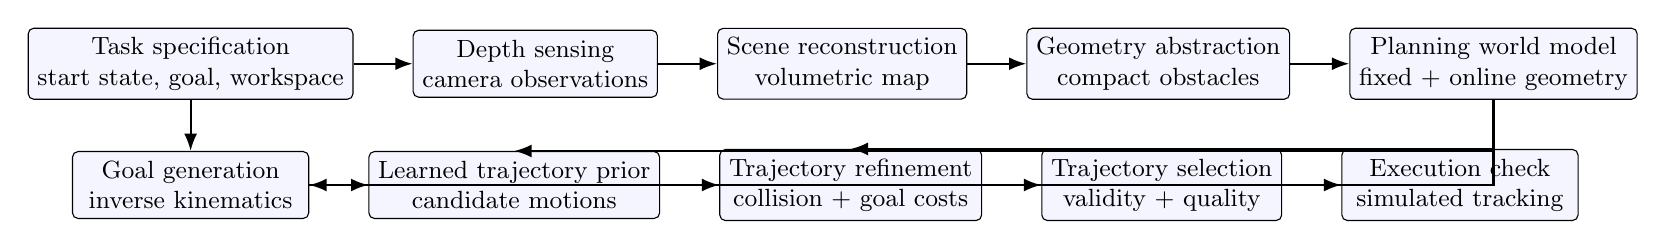
\begin{tikzpicture}[
        node distance=0.65cm and 0.75cm,
        box/.style={
            draw,
            rounded corners=2pt,
            align=center,
            minimum width=3.0cm,
            minimum height=0.85cm,
            font=\small,
            fill=blue!4
        },
        arrow/.style={-{Latex[length=2.2mm]}, thick}
    ]
        \node[box] (task) {Task specification\\start state, goal, workspace};
        \node[box, right=of task] (sense) {Depth sensing\\camera observations};
        \node[box, right=of sense] (recon) {Scene reconstruction\\volumetric map};
        \node[box, right=of recon] (geom) {Geometry abstraction\\compact obstacles};
        \node[box, right=of geom] (world) {Planning world model\\fixed + online geometry};

        \node[box, below=of task] (ik) {Goal generation\\inverse kinematics};
        \node[box, right=of ik] (learned) {Learned trajectory prior\\candidate motions};
        \node[box, right=of learned] (opt) {Trajectory refinement\\collision + goal costs};
        \node[box, right=of opt] (select) {Trajectory selection\\validity + quality};
        \node[box, right=of select] (exec) {Execution check\\simulated tracking};

        \draw[arrow] (task) -- (sense);
        \draw[arrow] (sense) -- (recon);
        \draw[arrow] (recon) -- (geom);
        \draw[arrow] (geom) -- (world);
        \draw[arrow] (task) -- (ik);
        \draw[arrow] (world.south) |- (ik.east);
        \draw[arrow] (ik) -- (learned);
        \draw[arrow] (world.south) |- (learned.north);
        \draw[arrow] (learned) -- (opt);
        \draw[arrow] (world.south) |- (opt.north);
        \draw[arrow] (opt) -- (select);
        \draw[arrow] (select) -- (exec);
    \end{tikzpicture}%
    }
    \caption{Final online deployment architecture.}
    \label{fig:system-architecture}
\end{figure}

The final system is organized as a perception-to-planning-to-execution pipeline. The task specification provides the robot's current state, the desired end-effector target, and the prior workspace model. The perception layer gathers depth observations from calibrated cameras and passes them to a reconstruction layer that estimates which parts of the workspace are occupied.

The reconstruction layer produces a volumetric representation of the scene. Because the learned planner does not operate directly on raw depth images, this representation is simplified into compact obstacle geometry. This abstraction step is deliberately conservative: it trades some geometric detail for a representation that can be evaluated quickly and reliably during planning.

The planning world model combines the known static environment with the newly reconstructed obstacle geometry. Before planning, the system checks whether the current robot state is still valid under this updated world model. If perception places obstacles on or very near the robot body, the system filters those artifacts so the planner does not reject the scene due to self-observation.

Goal generation converts the desired end-effector target into one or more feasible joint-space goals. This stage is necessary because the motion generator plans in the robot's configuration space, while the task is specified in end-effector space. Candidate goals are evaluated for target accuracy, collision validity, and proximity to the current state.

The planning module uses a learned trajectory prior to generate candidate motions, then refines and checks those motions using geometric collision costs, goal-reaching costs, and smoothness costs. A trajectory-selection stage chooses the best valid trajectory according to safety and quality criteria. Finally, a simulated execution layer replays the selected trajectory using a robot dynamics model and reports tracking behavior.

\section{Design Justification}

The system keeps a pretrained learned planner instead of retraining a new model for every obstacle configuration. This preserves the speed and quality of the learned motion prior while allowing the world model to change at runtime. The tradeoff is that online obstacles must be expressed in a representation compatible with the planner's collision model, and extreme scene distributions may still challenge a model trained on a finite set of examples.

The perception stack uses simulated depth before real hardware. This gives exact control over camera poses, obstacle placement, and robot state, making failures easier to debug. The tradeoff is realism: simulated depth is cleaner and more controlled than real sensor data. To reduce this gap, the system is structured around the same inputs a physical setup would provide: depth images, camera calibration, camera poses, and a robot state estimate.

A volumetric reconstruction layer was chosen because it provides a natural bridge between depth observations and collision-aware planning. It is more realistic than directly passing ground-truth obstacle shapes from simulation because it forces the planner to consume geometry through the same imperfect sensing channel that a real robot would use. The cost is additional computational overhead and representation-conversion work.

The final planning path converts dense reconstructed geometry into compact obstacle primitives. This is a conservative and simple interface to the collision checker, and it is easy to visualize, filter, and debug. The tradeoff is geometric fidelity: simplified primitives can over-approximate objects and remove free space. A more direct distance-field representation could preserve more detail, but it is harder to debug and depends more strongly on the quality of reconstruction gradients.

The planner uses a separate inverse-kinematics stage instead of asking the learned model to solve directly from end-effector pose alone. This separates task-space goal interpretation from motion generation. Sampling multiple goal candidates improves robustness to kinematic redundancy and obstacle placement. The tradeoff is extra latency, but it prevents the planner from being bottlenecked by a single poor or colliding goal configuration.

The system explicitly filters reconstructed geometry that collides with the current robot state. This is important because depth reconstruction can include the robot itself or produce artifacts near robot links, and a start state in collision causes planning to fail immediately. The tradeoff is that filtering may remove real nearby obstacles if perception is imperfect, so it should be treated as a guarded engineering fix rather than a substitute for calibrated robot segmentation.

Simulated trajectory replay was chosen as the final execution target instead of immediately commanding a physical robot. It verifies that the trajectory can be tracked by an articulated robot model with joint-level control, while avoiding the safety burden of hardware execution. The tradeoff is that controller-rate constraints, hardware latency, and real collision safety remain future work.

\section{Design Evolution}

At the proposal stage, the project goal was a real-world learned-planning deployment stack for a robot arm: capture depth from simulated or real cameras, reconstruct the scene, convert geometry into obstacles, plan a collision-free trajectory, and eventually execute on hardware. The initial idea treated perception and execution as direct extensions around the existing planner.

By the midterm implementation plan, the design became more concrete and phased. The main insight was that the learned planner still needed a joint-space goal, even when the task was described by an end-effector target. That turned online inverse kinematics from a nice-to-have into a core module. The plan also identified runtime obstacle injection as the cleanest first integration point, so the first phase used directly specified obstacles before adding depth reconstruction.

The next design step was to separate the system into independently testable phases. The first phase handled online planning with hand-authored obstacles. The second phase added simulated depth capture. The third phase added volumetric reconstruction. The fourth phase combined these pieces into a single perception-to-planning pipeline. Physical robot execution remained the target but was deferred because perception/planning integration and safety checks had to work first.

In the final implementation, the scope shifted from physical deployment to a complete simulated deployment pipeline. The final system captures depth, reconstructs occupied geometry, filters known static geometry and robot self-observations, converts the remaining geometry into compact obstacles, solves collision-aware inverse kinematics, plans with a pretrained learned motion model, and replays the selected trajectory in simulation. This was a practical pivot: it preserved the real deployment architecture while making the project testable in the available environment.

Several details changed because of empirical failure modes. First, directly specified obstacles were retained as a fallback because they isolate planner behavior from perception errors. Second, robot masking and self-geometry filtering were added because reconstructed depth could include the robot itself, falsely making the current state appear colliding. Third, start-state pruning was added because even after masking, small reconstruction artifacts near the arm could make the planner reject otherwise reasonable scenes. Fourth, the geometry abstraction evolved toward smaller merged primitives, which keeps the obstacle count manageable while representing clutter more flexibly than one large bounding volume.

The final architecture is therefore more modular than the initial idea. Instead of one monolithic ``online planner,'' it has explicit perception, reconstruction, geometry abstraction, goal generation, planning, and execution boundaries. That modularity made pivots easier: the system can run with directly specified obstacles, reconstructed obstacles, or a richer distance-field representation, and it can evaluate planning even when the real robot interface is not yet available.

\section{Reconstruction Benchmark Results}

The nvblox reconstruction benchmark evaluates the perception portion of the pipeline in isolation. For each trial, the two runtime cuboid obstacles in the warehouse scene were moved to random positions, two depth images were captured from the configured SAPIEN cameras, and nvblox reconstructed the occupied geometry. The reported reconstruction time excludes depth-image capture and measures only the nvblox integration, extraction, filtering, and box-conversion path. The benchmark used TSDF integration, sparse TSDF extraction, 5 cm voxels, known fixed-scene filtering, and robot self-geometry subtraction.

\begin{table}[htbp]
    \centering
    \begin{tabular}{l r}
        \hline
        Metric & Value \\
        \hline
        Iterations & 100 \\
        Random seed & 2 \\
        Depth frames per iteration & 2 \\
        Voxel size & 0.05 m \\
        Median nvblox reconstruction time & 0.301 s \\
        Mean nvblox reconstruction time & 0.301 s \\
        Reconstruction time standard deviation & 0.015 s \\
        Median depth-capture time, not included above & 2.801 s \\
        Median reconstructed-vs-ground-truth box IoU & 0.454 \\
        Mean reconstructed-vs-ground-truth box IoU & 0.449 \\
        Minimum reconstructed-vs-ground-truth box IoU & 0.336 \\
        Maximum reconstructed-vs-ground-truth box IoU & 0.521 \\
        \hline
    \end{tabular}
    \caption{nvblox reconstruction benchmark results for randomized EnvWarehouse runtime boxes.}
    \label{tab:nvblox-reconstruction-benchmark}
\end{table}

These results show that the reconstruction stage is fast enough for online replanning experiments in simulation: the median nvblox reconstruction time is about 301 ms, while depth capture is the larger cost at about 2.8 s and is excluded from the reported reconstruction timing. The median box IoU is 0.454, which indicates that the reconstructed geometry overlaps the ground-truth runtime boxes but remains approximate. This is expected because the pipeline reconstructs from two partial depth views, filters fixed warehouse geometry and robot geometry, and then compresses the remaining occupied voxels into axis-aligned cuboid primitives. The resulting boxes are therefore useful as conservative online obstacles for planning, but they should not be interpreted as exact object-shape recovery.

\section{Inverse-Kinematics Benchmark Results}

The inverse-kinematics benchmark evaluates the goal-generation stage of the pipeline. It uses the EnvWarehouse scene with the same two runtime cuboid obstacles used by the interactive warehouse demo, samples 100 end-effector goal poses from the validation dataset, and checks whether each IK method returns at least one collision-free joint goal that reaches the target pose within the configured tolerance. Median solution time is computed over the subset of benchmark problems for which at least one method succeeds; for any method that fails on one of those problems, its time for that problem is treated as infinite.

The benchmark output contained 80 eligible problems where at least one method found a solution. The original torch\_robotics method refers to the Adam-based IK implementation from commit \texttt{4cefb9f5cabf2940ba50b7258df4d045fd700012}. The current method uses the two-stage Levenberg--Marquardt solve followed by LBFGS collision refinement. The LM+Adam ablation keeps the Levenberg--Marquardt goal-pose solve but replaces the collision-refinement optimizer with Adam.

\begin{table}[htbp]
    \centering
    \begin{tabular}{l r r r}
        \hline
        Method & Successes & Success rate & Median solution time \\
        \hline
        Current two-stage LM + LBFGS & 67 / 80 & 83.75\% & 8.105 s \\
        Original torch\_robotics Adam & 78 / 80 & 97.50\% & 14.037 s \\
        LM + Adam refinement & 58 / 80 & 72.50\% & 6.044 s \\
        \hline
    \end{tabular}
    \caption{Inverse-kinematics benchmark results on 100 validation-set end-effector goals in EnvWarehouse with runtime obstacles. Metrics are reported over the 80 problems where at least one method succeeded.}
    \label{tab:ik-benchmark}
\end{table}

The original Adam-based torch\_robotics IK method solved the most eligible problems, succeeding on 78 of 80 cases, but it also had the slowest median solution time at 14.037 s. The current two-stage LM+LBFGS method was faster, with an 8.105 s median solution time, but solved fewer eligible problems. The LM+Adam ablation was the fastest among the three recorded methods, with a 6.044 s median solution time, but had the lowest success rate. These results suggest that the analytic Levenberg--Marquardt solve improves runtime, while the optimizer used for collision-aware refinement strongly affects robustness. The benchmark artifacts did not include completed rows for the Adam+LBFGS and Adam+Adam ablations, so they are not reported in Table~\ref{tab:ik-benchmark}.

\section{Planner Benchmark Results}

The planner benchmark evaluates trajectory generation in EnvWarehouse with extra runtime obstacles. The benchmark sampled 100 planning problems from the validation dataset, using each sample's start configuration, goal configuration, and end-effector goal pose. If the dataset goal configuration was in collision after adding the extra obstacles, the sampler attempted to recover a new collision-free goal configuration by solving inverse kinematics for the same end-effector goal pose. Four planner configurations were compared: MPD with 100, 10, and 1 sampled trajectories, and the \texttt{gp\_prior\_then\_guide} baseline, which performs gradient-based guidance without the diffusion model prior. For each solved trajectory, the benchmark also replayed the selected trajectory in SAPIEN and recorded median joint tracking error.

Metrics are reported over the 94 eligible problems where at least one method found a solution. If a method failed on one of these eligible problems, its solution time, tracking error, and path length for that problem were treated as infinite before computing medians. Planning time is the planner's reported inference time, path length is the selected joint-space path length, and tracking error is the median SAPIEN joint tracking error over the simulated execution.

\begin{table}[htbp]
    \centering
    \begin{tabular}{l r r r r}
        \hline
        Method & Successes & Median time & Median tracking error & Median path length \\
        \hline
        MPD, 100 samples & 94 / 94 & 0.831 s & 0.184 & 6.070 \\
        MPD, 10 samples & 90 / 94 & 0.662 s & 0.191 & 6.281 \\
        MPD, 1 sample & 68 / 94 & 0.595 s & 0.201 & 6.809 \\
        GP prior + guide & 56 / 94 & 1.095 s & 0.187 & 6.255 \\
        \hline
    \end{tabular}
    \caption{Planner benchmark results on 100 validation-set problems in \texttt{EnvWarehouseExtraObjectsV00}. Metrics are reported over the 94 problems where at least one planner succeeded, with failed attempts counted as infinite for median time, tracking error, and path length.}
    \label{tab:planner-benchmark}
\end{table}

The results show that the diffusion model prior substantially improves robustness. MPD with 100 samples solved all 94 eligible problems and had a median solution time of 0.831 s. Reducing MPD to 10 samples preserved most of the success rate, solving 90 of 94 eligible problems, and reduced median solution time to 0.662 s. With only one MPD sample, the median time dropped slightly to 0.595 s, but success fell to 68 of 94 eligible problems. The GP-prior baseline solved 56 of 94 eligible problems and had the slowest median solution time among the reported methods, which suggests that gradient-based guidance alone is less reliable than starting from diffusion-generated trajectory candidates.

The SAPIEN tracking results are similar across the successful methods, with median tracking errors between 0.184 and 0.201 radians in joint space. This indicates that once a planner returns a valid trajectory, the simulated controller can track it with comparable accuracy across methods. The main difference between planners is therefore not execution tracking, but how often they find a valid trajectory and how much sampling is needed to do so.

\end{document}
